Als alternativer Orientierungsalgorithmus zur lokalen Fluchtwegfindung kann der \emph{Bug-2-Algorithmus} dienen. Dieser stammt aus der Fahrzeugführung autonomer mobiler Roboter und ist ein reaktives Verfahren.
Dabei wird eine Wand-Detektion und -Verfolgung durchgeführt. Zusätzlich ist die Orientierung der Person lokal vorzuhalten. Das lokale Speichern des Headings einer Person widerspricht hier nicht den Anforderungen.

Bei dem Bug-2-Algorithmus wird eine sogenannte \emph{m-Linie} zwischen Person und dem Notausgang gebildet. Dazu wird die approximierte Position der Person genutzt. Die m-Linie kann als Luftlinie zwischen den beiden Punkten betrachtet werden.

\begin{figure}[!ht]
\centering
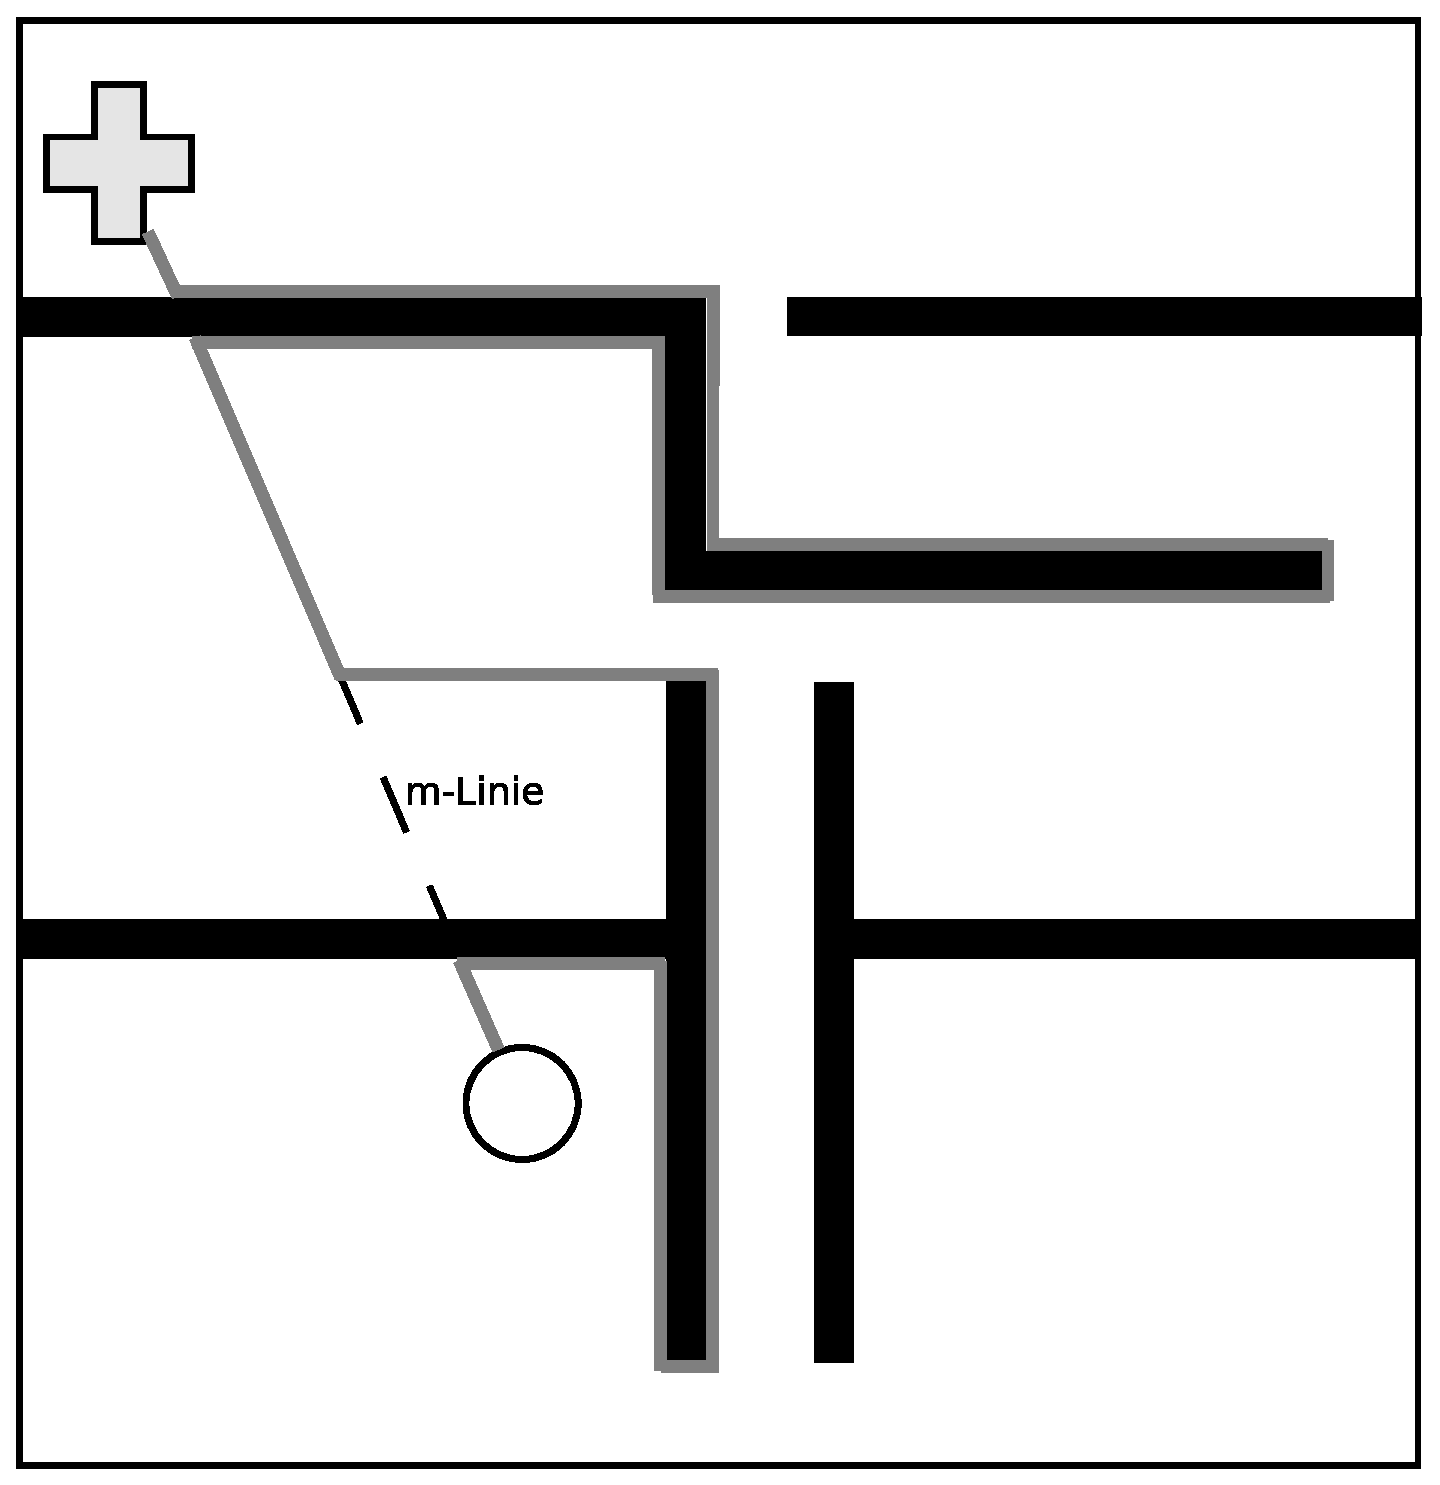
\includegraphics[height=0.35\textwidth]{evaluation/bug_2}
\caption{Veranschaulichung des Bug-2-Algorithmus}
\label{fig:bug_2}
\end{figure}

Abbildung \ref{fig:bug_2} zeigt schematisch einen Grundriss mit einer Person bzw. einem Agenten und einem Notausgang. Die \emph{m-Linie} ist gestrichelt dargestellt, die Wände schwarz.

Nach dem Auslösen der Flucht bewegt sich die Person entlang der m-Linie, bis eine Wand detektiert wird. Eine solche Detektion ist bereits bei dem \emph{random walk} implementiert worden. Es wird von der Person nun ein sogenanntes \emph{wall following} durchgeführt, bis die m-Linie näher am Notausgang passiert wird. Für diesen Schritt kann die initiale m-Linie lokal gespeichert werden oder falls möglich mit der approximierten Position eine neue m-Linie berechnet werden. Die Person bewegt sich erneut entlang der m-Linie.



\floatname{algorithm}{Algorithmus} 
\begin{algorithm}
\caption{Bug-2-Algorithmus}
\label{alg:bug_2}
\begin{algorithmic} 
\STATE last-heading $\leftarrow$ GET-HEADING()
\STATE exit-position $\leftarrow$ GET-NEAREST-EXIT()
\STATE m-line $\leftarrow$ LINE(exit-position, approx-position)
\WHILE{\textit{not rescued}}
\IF{not wall-in-front}
\STATE SET-HEADING(CALCULATE-HEADING(m-line))
\STATE FORWARD 1
\ELSE
\STATE follow-wall $\leftarrow$ true \hfill\emph{; wall detection}
\ENDIF
\WHILE{\textit{follow-wall}}
\IF{on-m-line}
\STATE follow-wall $\leftarrow$ false\hfill\emph{; abort wall following}
\ELSE
\STATE last-heading $\leftarrow$ FOLLOW-WALL(last-heading)\hfill\emph{; wall following}
\ENDIF
\ENDWHILE
\ENDWHILE
\end{algorithmic}
\end{algorithm}


